\chapter{Introduction}
\label{chap:introduction}
\setcounter{page}{1}
\pagenumbering{arabic}

In recent years, computer vision has made great progress. It's applied in many fields and people have achieved good results with it in some simple tasks, such as image classification~\cite{yu2017convolutional, lu2007survey}, image segmentation ~\cite{pham2000current} and face recognition~\cite{ahonen2006face, phillips1996feret}. Now people are no longer satisfied with these basic tasks, they also hope that computers can interpret pictures to obtain more information like humans, such as the attributes of objects,  the motion of objects, and the relationships between objects, etc. Thus people began to study some complex tasks such as Image Captioning ~\cite{hossain2019comprehensive},  Visual Question Answer~\cite{antol2015vqa}, and visual relationship detection (VRD). 

\begin{figure}[!htbp]
	\centering
	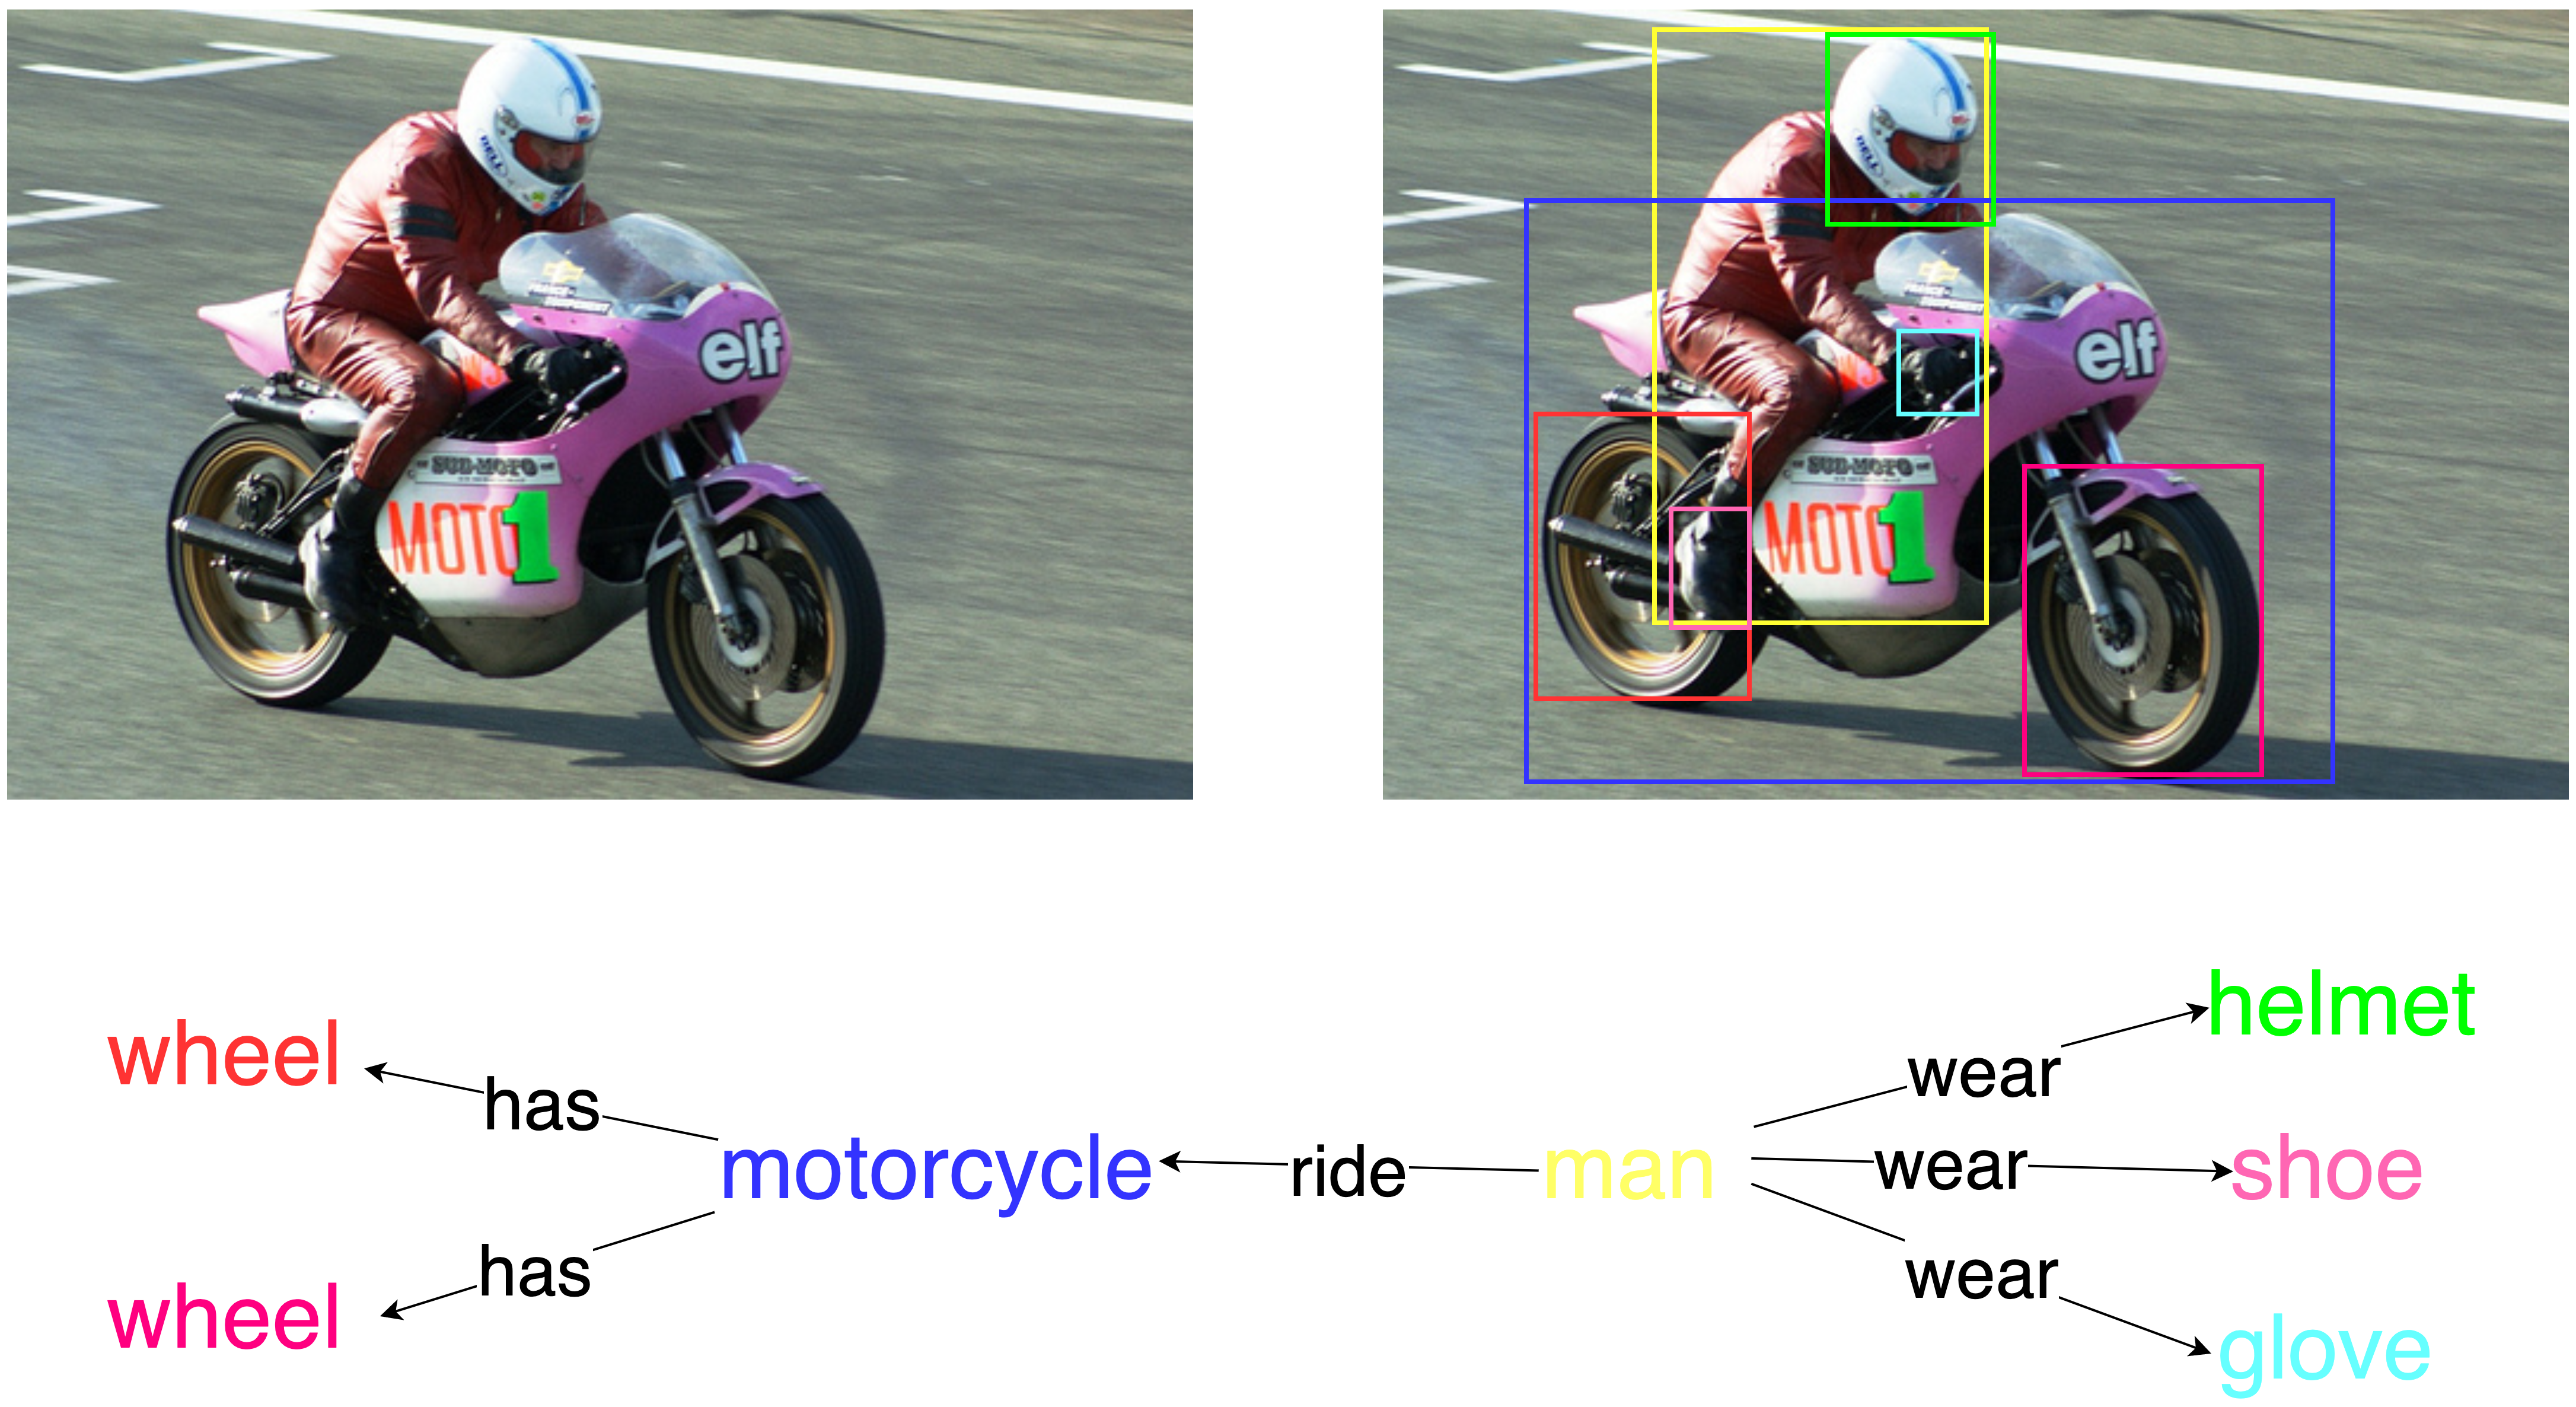
\includegraphics[width = 0.9 \textwidth]{figures/senen_graph.png}
	\caption[A example of visual relationship detection]
	{ A example of visual relationship detection: The upper left corner is the original input image, the upper right corner is the result of object detection, and the lower one is the relationship detection}
	\label{fig:sene}
\end{figure}

The visual relationship detection task needs to not only recognize the objects
in the images and their position, but also predict the relationship between the 
objects, and the relationship can be expressed as a triplet-Relationship: $\left \langle subject, predicate, object\right \rangle$. For example, in figure~\ref{fig:sene}, a VRD task includes identifying instances in the image: motorcycle, man, helmet, wheels, etc., as well as identifying the relationship between them, like $\left \langle man, ride, motorcycle\right \rangle$, $\left \langle man, wear, helmet\right \rangle$, $\left \langle motor, has, wheel\right \rangle$, etc..


\section{Motivation}

Visual relationship detection connects objects in images with predicates, and also connects low-level vision and high-level language (see Figure ~\ref{fig:vrd}). This means that visual relationship detection can provide high-level tasks, such as image captioning~\cite{hossain2019comprehensive} easier-to-understand information; It can also improve low-level tasks such as object detection using scene context. Visual relationship detection is an essential step to realize the target, that the computers can understand images as intelligently as humans.

\begin{figure}[!htbp]
	\centering
	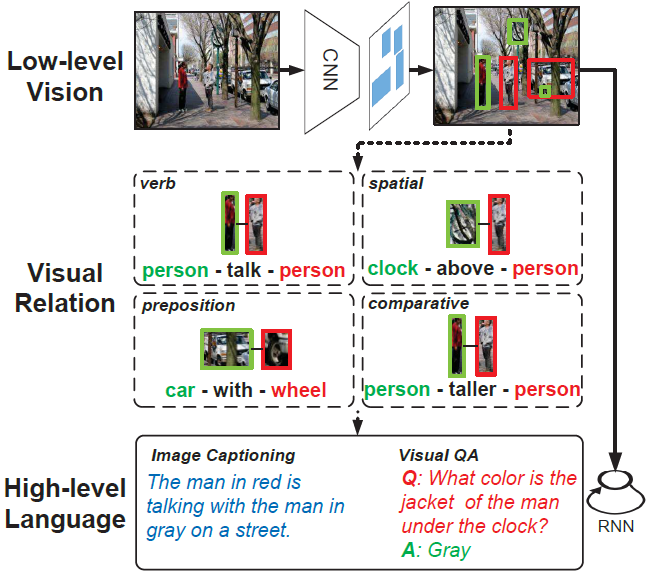
\includegraphics[width = 0.7 \textwidth]{figures/VRD.png}
	\caption[Connection between low-level vision and high-level vision]
	{ Visual relationship detection understands object interactions directly, which offer further semantic information for applications such as image captioning and QA. Figure obtained from ~\cite{zhang2017visual}}
	\label{fig:vrd}
\end{figure}

In recent years, with the proposal of the Transformer structure~\cite{vaswani2017attention}(see in section~\ref{section:transformer}), people have found that it not only achieves excellent performance in natural language processing tasks, but also has a very wide range of applications in computer vision, such as the DETR model~\cite{carion2020end} (see Figure ~\ref{fig:detr})proposed by Nicolas et al., using the Encoder-Decoder structure of the Transformer. The object detection effect of DETR is not inferior to Faster R-CNN~\cite{ren2016faster}. Thus we want to study the possibility of transformer structure in VRD problem. Our work is scene graph generation/visual relation detection, and object detection is the premise of scene graph generation/. Since the transformer can complete the object detection task well, we try to study whether it can continue to complete the remaining tasks of visual relation detection: predicts the interaction between objects.

In this thesis we utilise transformer encoder-decoder structure, aiming to solve problems regarding to Visual Relation Detection(VRD), meanwhile, as the attention mechanism is the most important part of Transformer, we need to pay more attention to it.

The motivaton for our task are mainly summarized as follows:

\begin{enumerate}[\qquad 1.]
	\item DETR has been proven to achieve good results in object detection with the use of Transformer. Since the object detection problems are solved well, we focus on finding a solution for relation detection through the transformer structure.
	\item When solving VRD's subtasks SGCLS and PREDCLS, we have the bounding boxes of the object and even the labels. In target detection, DETR uses a fixed learnable query to obtain a set of object features, and then matches the most likely object through a bipartite matching algorithm. But this learnable query is not suitable for the two subtasks we mentioned. It has no specific physical meaning, no correspondence with the real object and it cannot use the existing known information. Therefore, an object query is expected to designed that combines known information to achieve a one-to-one correspondence with objects.
	\item Attention mechanism is the fundamental principle of transformer, and we hope to obtain some information that is conducive to solving VRD problems by studying it. For example, through the attention between objects to explore whether they have a relationship, or through the study of the attention between relationship and object, to understand which two objects the relationship pays more attention to.
	\item The most important challenge is to predict the correct predicate, that describes the relation between two objects. To realise our goals, we designed a relation decoder, which helps to exploit semantic and spatial co-relation among various objects.
\end{enumerate}
 
 
\section{Contribution}

In this thesis, we provide  an efficient framework based on the  Transformer structure  for visual relationship detection that detects the interactions between objects in the image. The main work and contributions are summarized as following:
\begin{enumerate}[\qquad  1.]
	\item We propose a model based on the transformer structure, which solves the problems of predicate classification, scene graph classification and scene graph detection.
	\item An object query instead of learnable query is introduced to establish a direct connection with each object, so that we can make full use of the known information from predicate classification and scene graph classification, which makes every variable in the model more explanatory.
	\item A relation decoder is proposed, and establishes a new context propagation across relationships and objects, which improves the results of our tasks greatly.
\end{enumerate}


\section{Organization of the Thesis}
This thesis is structured as follows:

In Chapter~\ref{chap:relatedwork} , we will discuss about the related works. Some advanced researches and models about object detection and visual relationship detection are introduced briefly. We also demonstrate their contributions and limitations.

In Chapter ~\ref{chap:bg}, the theories about Transformer and other important models and algorithm such as Faster R-CNN , Hungarian matching and ranking loss  will be introduced.

In Chapter ~\ref{chap:framework}, the proposed framework will be shown in detail.

In Chapter ~\ref{chap:experiment}, the experimental results will be presented and analyzed in detail. Our proposed framework are evaluated on Visual Genome with three standard evaluation metrics.

In Chapter ~\ref{chap:conclusion}, we conclude our work finally and point out the future research direction.